\documentclass{beamer}
\usetheme{Boadilla}


\usepackage[utf8]{inputenc}
\usepackage{caption, subcaption}
\usepackage{amssymb, amsmath}
\usepackage{graphicx}


\title[Data-driven targeted gene panels]{Data-driven design of targeted gene panels for estimating immunotherapy biomarkers}
\author[Bradley and Cannings]{Jacob R. Bradley, Timothy I. Cannings}
\date{January 2021}
% \institute[]{University of Edinburgh}


\titlegraphic{
\includegraphics[height=.7cm]{figures/mims_logo.png}\hspace*{.5cm}~%

\includegraphics[height=.7cm]{figures/uoe_logo.png}\hspace*{.5cm}~
   
\includegraphics[height=1cm]{figures/igmm_logo.png}
}

\begin{document}

\begin{frame}
\titlepage
\end{frame}

\begin{frame}{Abstract}
\begin{enumerate}[I]
    \item Exome-wide biomarkers such as tumour mutation burden (TMB) are useful predictors of response to immunotherapy.
    \item While whole-exome sequencing directly measures TMB, its cost prevents it from being standard-of-care.
    \item We develop a data-driven framework both for selecting targeted gene panels and for using them to intelligently estimate immunotherapy biomarkers.
    \item To do this, we utilise an exome-wide generative model of mutation, whose structure can be chosen to reflect biological assumptions.
\end{enumerate}
\end{frame}


\begin{frame}
\frametitle{Outline}
\tableofcontents
\end{frame}

\section{Biological/Clinical Background}


\subsection{Cancer and immunotherapy}
\begin{frame}{Cancer is a disease of the genome}
Cancer arises when DNA in cells changes (mutates).
\begin{figure}[t!]
    \centering
    \begin{subfigure}[t]{0.45\textwidth}
        \centering
        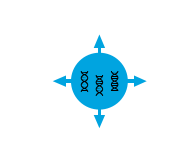
\includegraphics[height=1.5in]{figures/IC1.png}
        \caption{Non-cancer cell: Normal DNA.}
    \end{subfigure}
    ~ 
    \begin{subfigure}[t]{0.45\textwidth}
        \centering
        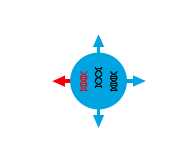
\includegraphics[height=1.5in]{figures/IC2.png}
        \caption{Cancer cell: Mutated DNA.}
    \end{subfigure}
\end{figure}
\end{frame}
\begin{frame}{Immunotherapy enables the immune system}
Immunotherapy 'releases the brakes' on the immune system in order for it to attack tumours.
\begin{figure}[t!]
    \centering
    \begin{subfigure}[t]{0.45\textwidth}
        \centering
        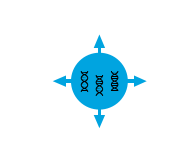
\includegraphics[height=1.5in]{figures/IC1.png}
        \caption{Low-damage cell: \textbf{unrecognisable} to immune system.}
    \end{subfigure}
    ~ 
    \begin{subfigure}[t]{0.45\textwidth}
        \centering
        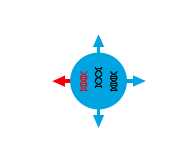
\includegraphics[height=1.5in]{figures/IC2.png}
        \caption{High-damage cell: \textbf{recognisable} to the immune system.}
    \end{subfigure}
\end{figure}
However, the immune system can only attack tumours that it recognises!
\end{frame}

\subsection{Exome-wide biomarkers}


\begin{frame}{Tumour mutation burden stratifies patients for immunotherapy response}
As a simple proxy for likelihood of immune response, we can use \textbf{tumour mutation burden}: the total count of non-synonymous mutations throughout the tumour exome. \\
~\\
Advantages:
\begin{enumerate}[I]
    \item Calculated from DNA sequencing only (compatible with liquid biopsy).
    \item Relevant across cancer types.
\end{enumerate}
Disadvantages:
\begin{enumerate}[I]
    \item Requires Whole-Exome Sequencing (WES) to measure directly. 
    \item Fails to incorporate other features of the immune environment.
\end{enumerate}



\end{frame}

\subsection{Targeted gene panels}

\begin{frame}{Targeted panels make genomic biomarkers viable}
Rather than the entire exome/genome, targeted gene panels sequence a \textbf{subset} of genes.

\begin{figure}[t!]
    \centering
    \begin{subfigure}[t]{0.45\textwidth}
        \centering
        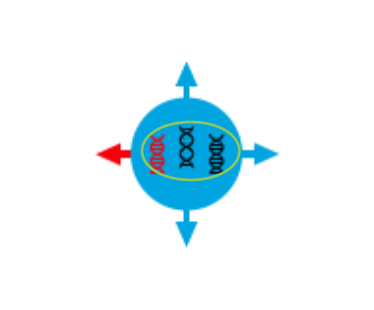
\includegraphics[height=1.5in]{figures/IC5.png}
        \caption{Whole-exome sequencing: \textbf{all genes} sequenced.}
    \end{subfigure}
    ~ 
    \begin{subfigure}[t]{0.45\textwidth}
        \centering
        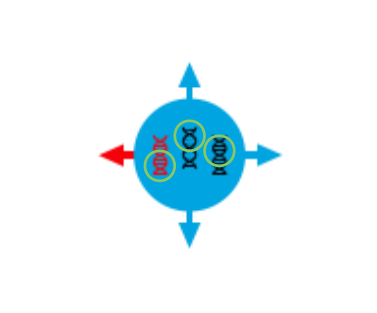
\includegraphics[height=1.5in]{figures/IC6.png}
        \caption{Targeted panel sequencing: \textbf{subset} of genes sequenced.}
    \end{subfigure}
\end{figure}

\end{frame}


\begin{frame}{Mutations and biomarkers: some notation}
We'll use $i,g,$ and $s$ to refer to:
\begin{enumerate}
    \item A sample $i$ (ranging from $i=1$ to $i=N$),
    \item A gene $g$ (belonging to some index set $G$),
    \item A 
\end{enumerate}
As a simplest proxy for likelihood of immune response, we can use tumour mutation burden:
\[
T = \sum_{g \in G} M_g
\]
where $G$ is the collection of genes in the genome, and $M_g$ is the number of mutations in gene $g$. \\
~\\
We want an estimator $\hat{T}$ that relies on observation of only some of the $M_g$s. For example in the case of a linear estimator, we may want 
\[\hat{T} = \sum_{g \in G} w_g M_g \]
with the coefficients $w_g$ sufficiently sparse.
\end{frame}

\section{Generative/predictive modelling framework}
\subsection{Generative models: what and why?}
\begin{frame}{What is a generative model of mutation?}
A generative model of mutation attempts to capture the underlying distribution of variants across the entire exome/genome. \\
~\\
A simple example (Poisson):
\begin{equation}
    M_{ig} \sim \mathrm{Poisson}(\lambda_g)
\end{equation}
\end{frame}

\begin{frame}{Why use generative models of mutation?}

\begin{enumerate}[I]
    \item Utilise known biology to inform the structure of the model.
    \item (Sometimes) make interpretable inferences.
    \item A predictive procedure: a means of getting from the learned generative model to predictions on unseen samples.  
\end{enumerate}

\end{frame}

\subsection{From generative models to predictive models}
\begin{frame}{Generative models to predictive models}
In order to realise the procedure above we need two things:
\begin{enumerate}[I]
    \item A generative model: a suitable joint distribution for the $M_g$s. 
    
    \item A predictive procedure: a means of getting from the learned generative model to predictions on unseen samples.
    \[\mathrm{E.g.} \quad \min_{\hat{T}}\{\mathbb{E}[(T-\hat{T})^2] + \lambda|\hat{T}|\}\]
\end{enumerate}

\end{frame}

\section{Application to non-small cell lung cancer}
\begin{frame}{Poisson-based generative model}

\begin{figure}[htbp]
\centering
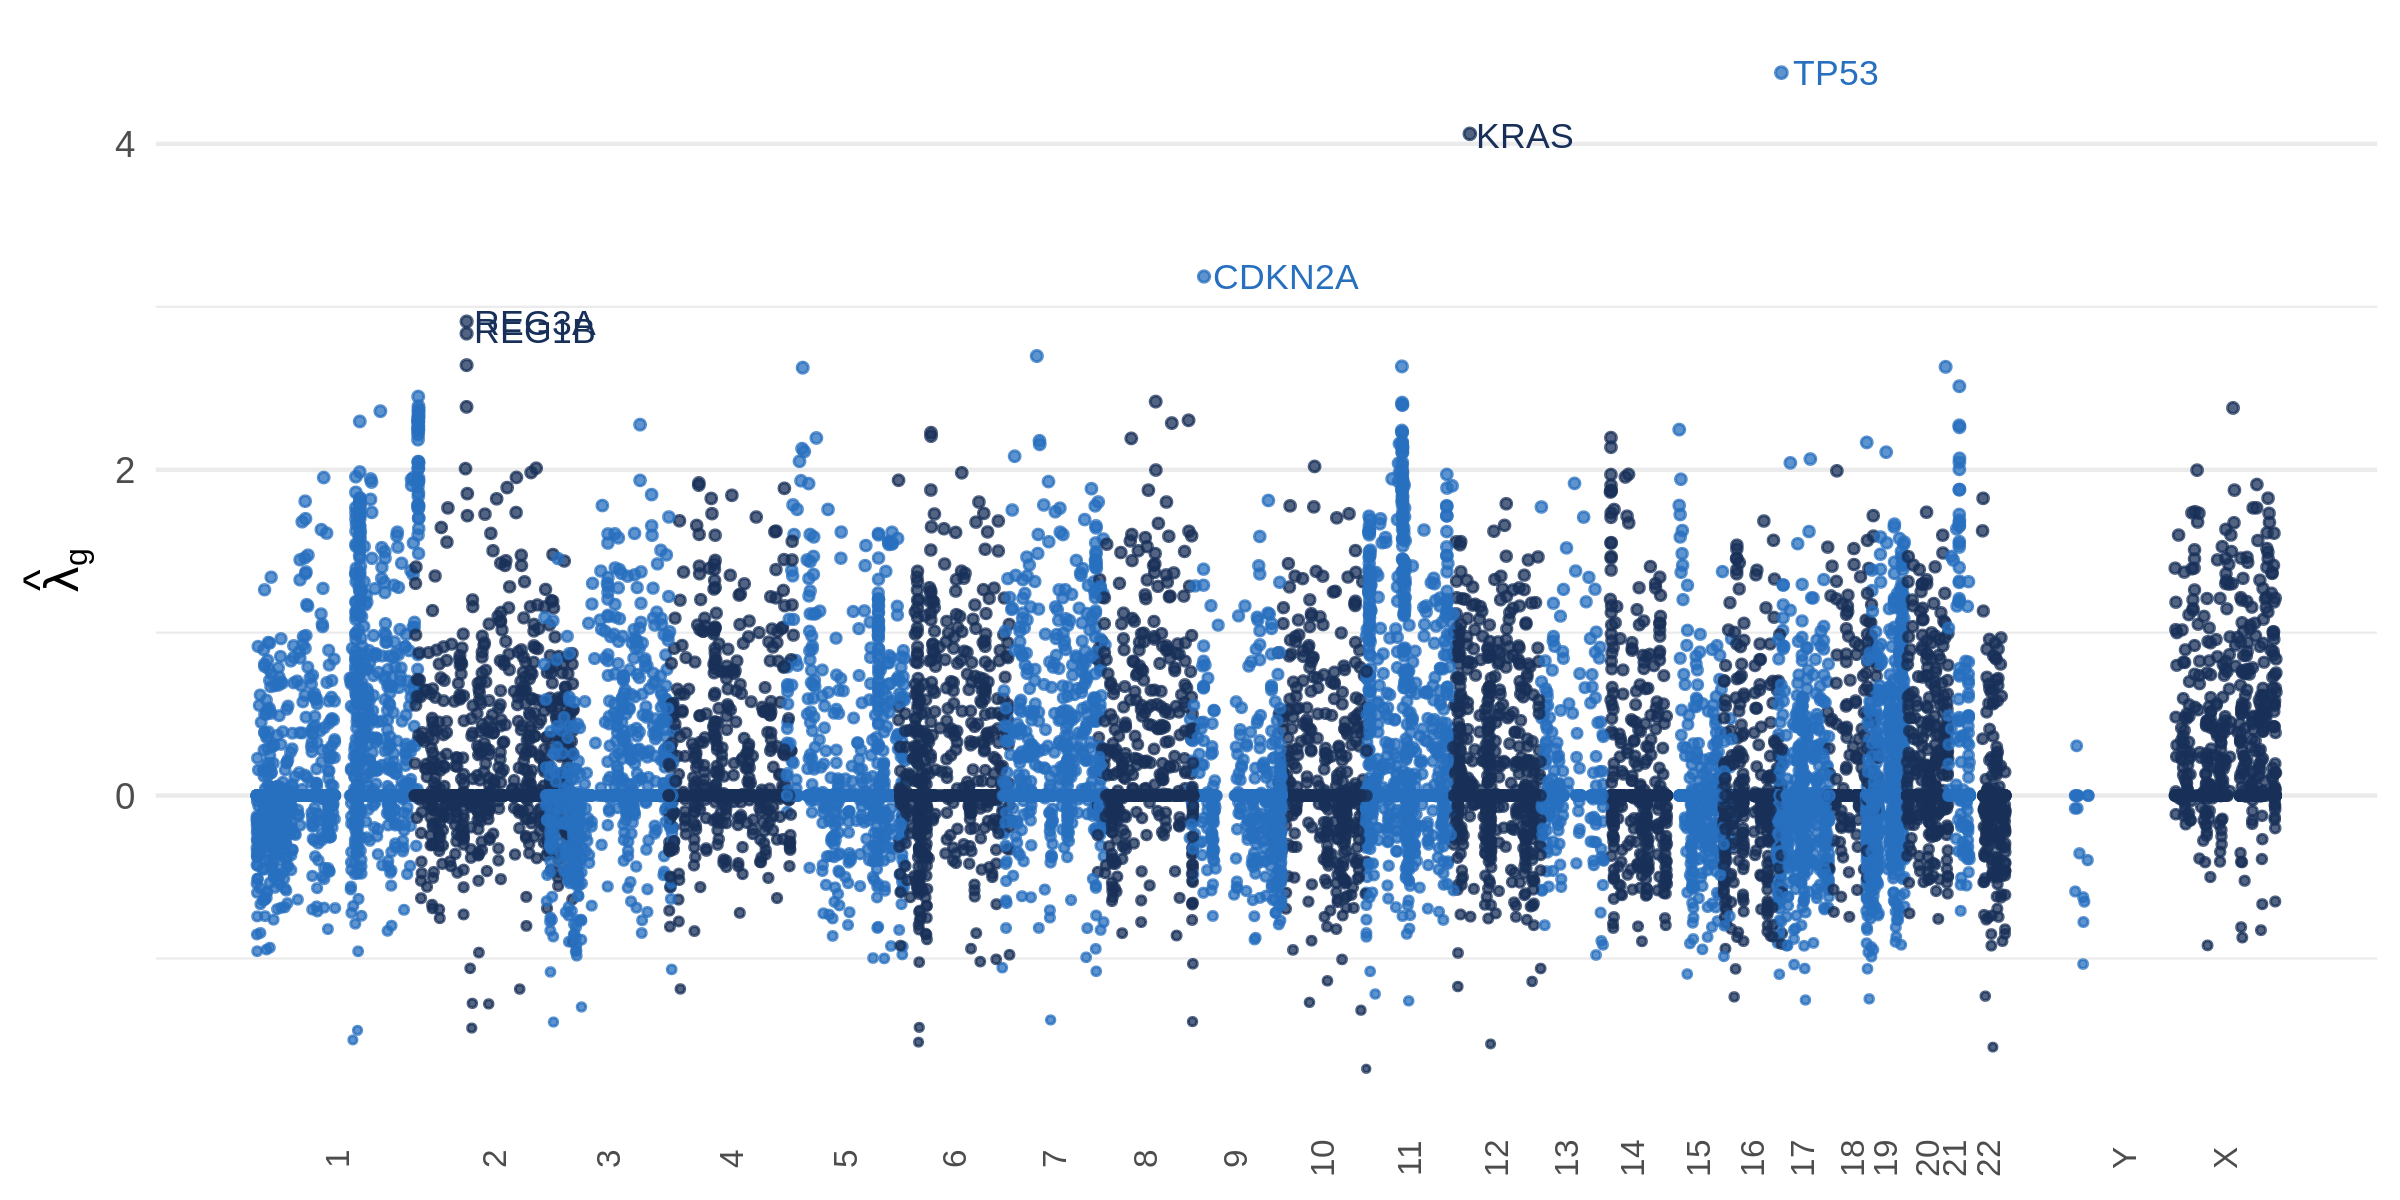
\includegraphics[width=4in]{figures/fig4.png}
\caption{ . \label{fig:3}}
\end{figure}
    
\end{frame}

\end{document}